\documentclass[11pt]{article}

\usepackage{neurips_2024_11pt}

\usepackage[utf8]{inputenc}
\usepackage[T1]{fontenc}
\usepackage{amsmath,amssymb,amsfonts,amsthm}
\usepackage{dsfont}
\usepackage{microtype}
\usepackage{booktabs}
\usepackage{array}
\usepackage{graphicx}
\usepackage{xcolor}
\usepackage{enumitem}
\usepackage{url}
\usepackage{tikz}
\usetikzlibrary{arrows.meta,positioning,shapes.geometric,fit,backgrounds,calc}
\usepackage{pgfplots}
\pgfplotsset{compat=1.18}
\usepgfplotslibrary{groupplots}
\usepackage[colorlinks=true,linkcolor=red!70!black,citecolor=blue!75!black,urlcolor=royalblue!85!black]{hyperref}
\AtBeginDocument{\setlength{\bibsep}{1.4pt}}

\theoremstyle{plain}
\newtheorem{theorem}{Theorem}[section]
\newtheorem{proposition}[theorem]{Proposition}
\newtheorem{corollary}[theorem]{Corollary}
\theoremstyle{definition}
\newtheorem{definition}[theorem]{Definition}

% Unified, collision-free notation macros
\newcommand{\piref}{\pi_{\mathrm{ref}}}
\newcommand{\pitheta}{\pi_{\theta}}
\newcommand{\pithetastar}{\pi_{\theta^*}}
\newcommand{\LDPO}{\mathcal{L}_{\mathrm{DPO}}}
\newcommand{\Racc}{\mathcal{R}}
\newcommand{\Racctilde}{\widetilde{\mathcal{R}}}
\newcommand{\Ind}{\mathds{1}}
\newcommand{\E}{\mathbb{E}}
\newcommand{\CtoC}{\mathrm{C{\to}C}}
\newcommand{\CtoI}{\mathrm{C{\to}I}}
\newcommand{\ItoC}{\mathrm{I{\to}C}}
\newcommand{\ItoI}{\mathrm{I{\to}I}}

\definecolor{navybox}{HTML}{1E3A5F}
\definecolor{slatefill}{HTML}{F0F4F8}
\definecolor{tealbox}{HTML}{1D6F72}
\definecolor{amberbox}{HTML}{C05621}
\definecolor{crimson}{HTML}{C53030}
\definecolor{forest}{HTML}{2F855A}
\definecolor{royalblue}{HTML}{2B6CB0}
\definecolor{colabGold}{HTML}{F9AB00}
\definecolor{colabOrange}{HTML}{E8710A}
\definecolor{githubBlack}{HTML}{181717}

\pgfplotsset{
  neuripsplot/.style={
    axis x line*=bottom,
    axis y line*=left,
    tick align=outside,
    major tick length=2.4pt,
    axis line style={black!75, line width=0.55pt},
    tick style={black!70, line width=0.5pt},
    ymajorgrids=true,
    xmajorgrids=false,
    grid style={densely dotted, gray!38, line width=0.45pt},
    label style={font=\small},
    tick label style={font=\footnotesize},
    title style={font=\small\bfseries, yshift=1pt},
  }
}

\newcommand{\colaburl}{https://colab.research.google.com/drive/15joRmKadegeO1RI3dHm79bjFBoDKGjWD?usp=sharing}
\newcommand{\githuburl}{https://github.com/aayushmanda/Pref_Ranking/}
\newcommand{\officialurl}{https://github.com/angie-chen55/pref-learning-ranking-acc}

\DeclareRobustCommand{\colabicon}{%
  \tikz[baseline=0ex, line cap=butt]{%
    \draw[colabGold, line width=0.28ex] (0,0.58ex) ++(42:0.46ex) arc (42:125:0.46ex);
    \draw[colabOrange, line width=0.28ex] (0,0.58ex) ++(125:0.46ex) arc (125:235:0.46ex);
    \draw[colabGold, line width=0.28ex] (0,0.58ex) ++(235:0.46ex) arc (235:318:0.46ex);
    \draw[colabOrange, line width=0.28ex] (0.98ex,0.58ex) ++(125:0.46ex) arc (125:305:0.46ex);
    \draw[colabGold, line width=0.28ex] (0.98ex,0.58ex) ++(-55:0.46ex) arc (-55:125:0.46ex);
  }%
}

\DeclareRobustCommand{\githubicon}{%
  \tikz[baseline=-0.08ex, x=0.68ex, y=0.68ex]{%
    \fill[githubBlack] (0,0.82) circle (1.0);
    \fill[white]
      (-0.21,-0.16) -- (-0.21,0.20)
      .. controls (-0.48,0.14) and (-0.55,0.34) .. (-0.66,0.40)
      .. controls (-0.70,0.42) and (-0.64,0.46) .. (-0.56,0.43)
      .. controls (-0.46,0.39) and (-0.42,0.26) .. (-0.21,0.29)
      -- (-0.21,0.40)
      .. controls (-0.48,0.45) and (-0.64,0.62) .. (-0.64,0.90)
      .. controls (-0.64,1.05) and (-0.58,1.16) .. (-0.49,1.25)
      .. controls (-0.53,1.36) and (-0.53,1.48) .. (-0.46,1.56)
      .. controls (-0.36,1.56) and (-0.25,1.48) .. (-0.18,1.40)
      .. controls (-0.06,1.43) and (0.06,1.43) .. (0.18,1.40)
      .. controls (0.25,1.48) and (0.36,1.56) .. (0.46,1.56)
      .. controls (0.53,1.48) and (0.53,1.36) .. (0.49,1.25)
      .. controls (0.58,1.16) and (0.64,1.05) .. (0.64,0.90)
      .. controls (0.64,0.62) and (0.48,0.45) .. (0.21,0.40)
      -- (0.21,-0.16) -- cycle;
  }%
}

\DeclareRobustCommand{\prefnb}{%
  \href{\colaburl}{\colabicon\,\texttt{Colab}}%
}

\DeclareRobustCommand{\ghrepo}{%
  \href{\githuburl}{\githubicon\,\texttt{GitHub}}%
}

\DeclareRobustCommand{\officialrepo}{%
  \href{\officialurl}{\githubicon\,\texttt{angie-chen55/\allowbreak pref-learning-ranking-acc}}%
}

\DeclareRobustCommand{\officialreposhort}{%
  \href{\officialurl}{\githubicon\,\texttt{Official Repo}}%
}

\title{Preference Learning Algorithms Do Not Learn Preference Rankings:\\[4pt]
{\Large An Empirical and Theoretical Investigation of Chen et al.\ (2024)}}

\author{%
  Aayushman\\[4pt]
  {\normalfont\small \href{\githuburl}{\githubicon\,\texttt{github.com/aayushmanda/Pref\_Ranking}} \quad\textbullet\quad \prefnb{}}
}

\begin{document}

\maketitle

\begin{abstract}
Direct Preference Optimization (DPO) steadily reduces training loss across epochs, so it is natural to expect a DPO-trained language model to assign higher sequence probability to preferred responses than to dispreferred ones. Yet \citet{chen2024preference} show that DPO models achieve pairwise ranking accuracy below $60\%$ and correct fewer than $10\%$ of reference-model ranking errors before validation overfitting. In this report, we investigate why loss minimization fails to fix pairwise rankings through theoretical analysis, an audit of the authors' official codebase (\officialreposhort{}), floating-point precision checks, and full-parameter \texttt{GPT-2} (124M) experiments (\prefnb{}) on $16{,}000$ human preference dialogues \citep{bai2022training}. Because the DPO objective shifts policy log-ratios by the frozen reference model's initial log-ratio, pairs that are strongly misranked by the reference model achieve positive reward margins and vanishing sigmoid gradients long before their sequence rankings flip. Auditing the official scripts further shows that two evaluation bugs substantially overstate the reported idealized-accuracy gap, while standard \texttt{float32} loss evaluation and \texttt{bfloat16} master weights introduce severe rounding errors in the tail and during parameter updates. Across five epochs of DPO training, mean probe loss drops by $45\%$, yet only $4.2\%$ of initially misranked pairs flip at the best validation checkpoint ($6.9\%$ by Epoch~$5$). In fact, the hardest reference-misranked pairs reach the lowest median loss ($0.22$) of any subset while flipping $0\%$ of the time, matching the exact theoretical flipping threshold across all $1{,}000$ evaluated pairs.
\end{abstract}

% =========================================================================
\section{Introduction}
\label{sec:intro}
% =========================================================================

Reinforcement Learning from Human Feedback \citep[RLHF,][]{stiennon2020learning,bai2022training} and Direct Preference Optimization \citep[DPO,][]{rafailov2023direct} align language models using pairwise human comparisons $(x, y_w, y_l)$, where $y_w$ is preferred over $y_l$ for prompt $x$. Because DPO minimizes a binary cross-entropy loss over the relative log-probabilities of $y_w$ and $y_l$, a steady decrease in training loss is commonly assumed to imply that $\pitheta(y_w \mid x) > \pitheta(y_l \mid x)$ on most training and validation pairs.

\citet{chen2024preference} test this assumption directly via \emph{ranking accuracy} $\Racc(\pitheta)$, the fraction of pairs on which $\pitheta$ assigns higher sequence probability to $y_w$ than to $y_l$. They report four main claims, which we evaluate side by side with our findings in Table~\ref{tab:claims_roadmap}.

\begin{table}[t]
  \centering
  \caption{\textbf{Summary of the Four Claims in \citet{chen2024preference} and Our Main Findings.}}
  \label{tab:claims_roadmap}
  \small
  \renewcommand{\arraystretch}{1.18}
  \setlength{\tabcolsep}{5pt}
  \begin{tabular*}{\textwidth}{@{\extracolsep{\fill}}l >{\raggedright\arraybackslash}p{4.3cm} >{\raggedright\arraybackslash}p{6.0cm} c@{}}
    \toprule
    \textbf{Claim} & \textbf{Claim in \citet{chen2024preference}} & \textbf{Our Finding} & \textbf{Section} \\
    \midrule
    \textbf{Claim 1} & Pretrained and SFT reference policies satisfy $\Racc(\piref) < 60\%$. & Confirmed ($46.6\%$ Pre-SFT, $48.1\%$ Post-SFT on \texttt{GPT-2}). Length spread ($\ell_w - \ell_l \ge +86$ words in the top $5\%$) penalizes raw $\log \piref(y_w \mid x)$ and creates a heavy $c > 0$ tail. & \S\ref{sec:setup}, \S\ref{sec:results} \\
    \addlinespace[3pt]
    \textbf{Claim 2} & Aligned models fall $19\text{--}59$\,pp below idealized accuracy $\Racc^*$. & Overstated. Clamping $4/4$ votes to $\hat{p} = 0.999$ inflates the flip cutoff nearly $5\times$ ($69.1$ vs.\ $13.9$), and missing \texttt{np.exp} in \texttt{rlhf\_minimizer\_client.py} inverts length penalties. & \S\ref{sec:theory}, \S\ref{sec:critique} \\
    \addlinespace[3pt]
    \textbf{Claim 3} & DPO loss falls steadily, yet under $10\%$ of reference errors flip before overfitting ($t^*$). & Confirmed. Mean probe $\LDPO$ falls $0.6931 \to 0.4690$ at $t^* = 1{,}100$ ($0.3807$ at Epoch~$5$), yet only $4.24\%$ ($22/519$) of misranked pairs flip at $t^*$ ($6.94\%$ at Epoch~$5$). & \S\ref{sec:critique}, \S\ref{sec:results} \\
    \addlinespace[3pt]
    \textbf{Claim 4} & Flipping a misranked pair requires $\LDPO \le -\log\sigma(\beta c)$, blocking large-$c$ flips. & Confirmed ($1{,}000/1{,}000$ exact match). Hard pairs ($c > 100$) reach the lowest median loss ($0.217$) yet flip $0.0\%$. Naive \texttt{float32} loss also causes $85.1\%$ tail false flips. & \S\ref{sec:numerical}, \S\ref{sec:results} \\
    \bottomrule
  \end{tabular*}
\end{table}

Our goal is to separate genuine properties of the DPO objective from implementation and numerical artifacts, and to present a clean, self-contained empirical verification in \prefnb{}. Section~\ref{sec:theory} introduces unified notation and derives the exact flipping threshold $f(c)$. Section~\ref{sec:critique} analyses gradient saturation under $\LDPO$ and shows why two evaluation choices in \citet{chen2024preference} inflate $\Racc^*$. Section~\ref{sec:setup} describes our full-parameter \texttt{GPT-2} pipeline, contrasts four bugs in the official codebase against our fixes, and quantifies response-length dispersion across $16{,}000$ dialogue pairs. Section~\ref{sec:numerical} presents two floating-point failure modes we resolved during implementation (\texttt{log1p} tail underflow and \texttt{bfloat16} master-weight rounding). Section~\ref{sec:results} presents our 5-epoch SFT-to-DPO results and four empirical observations, and Section~\ref{sec:discussion} connects these results to reference-free and on-policy alignment objectives.

% =========================================================================
\section{Notation, Problem Formulation, and Flipping Threshold}
\label{sec:theory}
% =========================================================================

\paragraph{Notation.}
For a prompt $x$ and response $y = (y_1, \dots, y_\ell)$ of token length $\ell$, an autoregressive policy $\pitheta$ assigns sequence log-likelihood $\log \pitheta(y \mid x) = \sum_{t=1}^{\ell} \log \pitheta(y_t \mid x, y_{<t}) < 0$. On a preference pair $(x, y_w, y_l)$ with token lengths $\ell_w$ and $\ell_l$ and frozen reference policy $\piref$, three scalar quantities govern DPO training and ranking:
\begin{align}
  \delta_\theta &\triangleq \log \frac{\pitheta(y_w \mid x)}{\pitheta(y_l \mid x)},
  \qquad\qquad
  c \triangleq \log \frac{\piref(y_l \mid x)}{\piref(y_w \mid x)}, \nonumber \\[3pt]
  u_\theta &\triangleq \beta(\delta_\theta + c)
  = \beta \log \frac{\pitheta(y_w \mid x)}{\piref(y_w \mid x)}
  - \beta \log \frac{\pitheta(y_l \mid x)}{\piref(y_l \mid x)},
  \label{eq:three_quantities}
\end{align}
where $\beta > 0$ is the KL temperature. Here $\delta_\theta$ is the \emph{policy log-ratio} ($\delta_\theta \ge 0$ means $\pitheta$ ranks $y_w$ above $y_l$), $c$ is the \emph{reference log-ratio} (RMLR, with $y_l$ in the numerator so $c \le 0$ means $\piref$ is initially correct and $c > 0$ means $\piref$ misranks the pair), and $u_\theta$ is the \emph{DPO reward margin}. Because DPO initializes $\theta_0 = \theta_{\mathrm{ref}}$, every pair starts at $\delta_{\theta_0} = -c$, $u_{\theta_0} = 0$, and Step-$0$ loss $\ln 2 \approx 0.6931$.

\begin{definition}[Raw and Length-Normalized Ranking Accuracy]
\label{def:rank_acc}
The raw ($\Racc$) and length-normalized ($\Racctilde$) ranking accuracies of $\pitheta$ over a dataset $\mathcal{D}$ are
\begin{equation}
  \Racc(\pitheta) = \E_{\mathcal{D}}\big[\Ind\{\delta_\theta \ge 0\}\big],
  \qquad
  \Racctilde(\pitheta) = \E_{\mathcal{D}}\!\left[\Ind\!\left\{\frac{\log \pitheta(y_w \mid x)}{\ell_w} \ge \frac{\log \pitheta(y_l \mid x)}{\ell_l}\right\}\right].
  \label{eq:ranking_acc}
\end{equation}
\end{definition}

\paragraph{Reward Accuracy Versus Ranking Accuracy.}
Benchmarks such as RewardBench evaluate DPO's implicit reward $\hat{r}_\theta(x, y) = \beta \log \frac{\pitheta(y \mid x)}{\piref(y \mid x)}$, which marks a pair correct whenever $u_\theta > 0$, or equivalently $\delta_\theta > -c$. If $\piref$ misranks a pair with $c = 100$ ($\delta_{\theta_0} = -100$) and DPO raises $\delta_\theta$ to $-80$, implicit reward accuracy is $1$ ($u_\theta = 20\beta > 0$), yet $\pitheta(y_l \mid x)$ remains $e^{80}$ times larger than $\pitheta(y_w \mid x)$, so $\Racc = 0$. Because autoregressive decoding samples from $\pitheta(y \mid x)$ rather than $\pitheta(y \mid x)/\piref(y \mid x)$, $\Racc$ reflects the policy's actual sequence ordering.

\paragraph{DPO Loss, Idealized Accuracy, and Flipping Threshold.}
On empirical preference data, DPO minimizes $\LDPO(\pitheta) = -\log \sigma(u_\theta) = \log(1 + e^{-u_\theta})$, where $\sigma(u) = (1 + e^{-u})^{-1}$. If ground-truth human preferences follow a Bradley-Terry probability $p = \mathbb{P}(y_w \succ y_l \mid x) \in (0.5, 1)$ \citep{bradley1952rank}, minimizing the population cross-entropy $-p \log \sigma(u_\theta) - (1 - p)\log(1 - \sigma(u_\theta))$ yields $\sigma(u_{\theta^*}) = p$, or $\delta_{\theta^*} = \frac{1}{\beta}\log\frac{p}{1-p} - c$. Taking the indicator $\delta_{\theta^*} > 0$ gives the idealized ranking accuracy \citep[Theorem~3.1 and Corollary~3.3,][]{chen2024preference}:
\begin{equation}
  \Racc^*(\piref) = \E_{\mathcal{D}}\!\left[\Ind\!\left\{\frac{1}{\beta}\log\frac{p}{1 - p} > c\right\}\right].
  \label{eq:idealized_acc}
\end{equation}
On single-rater binary labels ($\hat{p} = 1$), substituting $\delta_\theta \ge 0$ directly into $u_\theta = \beta(\delta_\theta + c)$ characterizes when a pair is ranked correctly at any parameter vector $\theta$.

\begin{theorem}[Exact Flipping Threshold, Thm.~4.1 in \citet{chen2024preference}]
\label{thm:flip_threshold}
For any preference pair $(x, y_w, y_l)$ with reference log-ratio $c$,
\begin{equation}
  \delta_\theta \ge 0
  \iff u_\theta \ge \beta c
  \iff \LDPO(\pitheta) \le f(c) \triangleq -\log \sigma(\beta c) = \log(1 + e^{-\beta c}).
  \label{eq:thm4_1}
\end{equation}
\end{theorem}
\begin{proof}
Since $\beta > 0$ and $u \mapsto -\log \sigma(u)$ is strictly decreasing on $\mathbb{R}$, $\delta_\theta \ge 0 \iff \beta(\delta_\theta + c) \ge \beta c \iff -\log \sigma(u_\theta) \le -\log \sigma(\beta c)$.
\end{proof}

\begin{figure}[t]
  \centering
  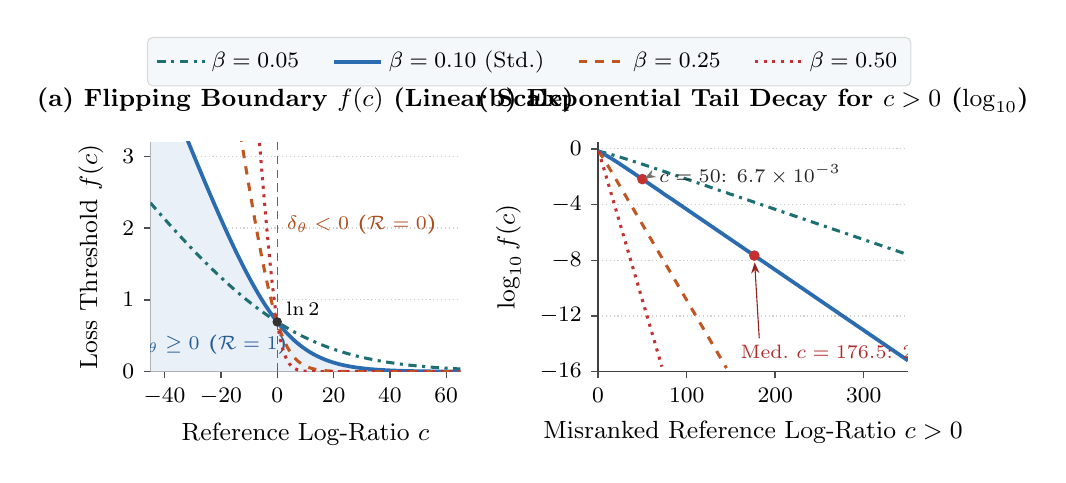
\begin{tikzpicture}
    \begin{groupplot}[
      group style={group size=2 by 1, horizontal sep=1.75cm},
      height=4.5cm,
      width=0.455\textwidth,
      neuripsplot,
    ]
    \nextgroupplot[
      title={(a) Flipping Boundary $f(c)$ (Linear Scale)},
      xlabel={Reference Log-Ratio $c$},
      ylabel={Loss Threshold $f(c)$},
      xmin=-45, xmax=65,
      ymin=0, ymax=3.2,
      xtick={-40,-20,0,20,40,60},
      ytick={0,1,2,3},
      legend to name=fig1sharedlegend,
      legend columns=4,
      legend style={font=\footnotesize, draw=gray!30, fill=slatefill!65, rounded corners=2pt, inner sep=3pt, /tikz/every even column/.append style={column sep=0.35cm}}
    ]
      \path[fill=royalblue!10] (axis cs:-45,0) -- (axis cs:-45,3.2) -- (axis cs:-31.6,3.2)
        -- plot[domain=-31.6:65, samples=80] (\x, {ln(1 + exp(-0.1*\x))})
        -- (axis cs:65,0) -- cycle;
      \node[font=\scriptsize\bfseries, text=royalblue!85!black] at (axis cs:-23,0.38) {$\delta_\theta \ge 0$ ($\Racc=1$)};
      \node[font=\scriptsize\bfseries, text=amberbox!90!black] at (axis cs:30,2.05) {$\delta_\theta < 0$ ($\Racc=0$)};

      \addplot[line width=1.1pt, tealbox, dashdotted, samples=120, domain=-45:65] {ln(1 + exp(-0.05*x))};
      \addlegendentry{$\beta = 0.05$}
      \addplot[line width=1.35pt, royalblue, samples=120, domain=-45:65] {ln(1 + exp(-0.10*x))};
      \addlegendentry{$\beta = 0.10$ (Std.)}
      \addplot[line width=1.1pt, amberbox, dashed, samples=120, domain=-15:65] {ln(1 + exp(-0.25*x))};
      \addlegendentry{$\beta = 0.25$}
      \addplot[line width=1.1pt, crimson, dotted, samples=120, domain=-8:65] {ln(1 + exp(-0.50*x))};
      \addlegendentry{$\beta = 0.50$}

      \draw[densely dashed, black!60, line width=0.5pt] (axis cs:0,0) -- (axis cs:0,3.2);
      \filldraw[black!80] (axis cs:0,0.6931) circle (1.5pt);
      \node[font=\scriptsize, anchor=south west, inner sep=1.5pt] at (axis cs:1.5,0.72) {$\ln 2$};

    \nextgroupplot[
      title={(b) Exponential Tail Decay for $c > 0$ ($\log_{10}$)},
      xlabel={Misranked Reference Log-Ratio $c > 0$},
      ylabel={$\log_{10} f(c)$},
      xmin=0, xmax=350,
      ymin=-16, ymax=0.5,
      xtick={0,100,200,300},
      ytick={0,-4,-8,-12,-16}
    ]
      \addplot[line width=1.1pt, tealbox, dashdotted, samples=100, domain=0:350]
        {ifthenelse(0.05*x < 8, log10(ln(1 + exp(-0.05*x))), -0.05*x*0.434294)};
      \addplot[line width=1.35pt, royalblue, samples=100, domain=0:350]
        {ifthenelse(0.10*x < 8, log10(ln(1 + exp(-0.10*x))), -0.10*x*0.434294)};
      \addplot[line width=1.1pt, amberbox, dashed, samples=80, domain=0:145]
        {ifthenelse(0.25*x < 8, log10(ln(1 + exp(-0.25*x))), -0.25*x*0.434294)};
      \addplot[line width=1.1pt, crimson, dotted, samples=60, domain=0:72]
        {ifthenelse(0.50*x < 8, log10(ln(1 + exp(-0.50*x))), -0.50*x*0.434294)};

      \filldraw[crimson] (axis cs:50,-2.174) circle (1.7pt);
      \node[font=\scriptsize, anchor=west, text=black!85] at (axis cs:58,-1.85) {$c=50$: $6.7\times 10^{-3}$};
      \draw[-{Stealth[length=1.4mm]}, thin, black!55] (axis cs:58,-1.95) -- (axis cs:52.5,-2.14);

      \filldraw[crimson] (axis cs:176.45,-7.665) circle (1.7pt);
      \node[font=\scriptsize, anchor=west, text=crimson!90!black] at (axis cs:150,-14.5) {Med.\ $c=176.5$: $2.2\times 10^{-8}$};
      \draw[-{Stealth[length=1.4mm]}, thin, crimson!75!black] (axis cs:182,-13.6) -- (axis cs:176.8,-8.15);
    \end{groupplot}
    \node[anchor=south] at ($(group c1r1.north)!0.5!(group c2r1.north) + (0,0.58cm)$)
      {\pgfplotslegendfromname{fig1sharedlegend}};
  \end{tikzpicture}
  \caption{\textbf{Analytical Flipping Threshold $f(c) = -\log\sigma(\beta c)$ (Theorem~\ref{thm:flip_threshold}).} \textbf{(a)} Shaded region marks $\LDPO \le f(c)$ at $\beta = 0.10$, where $\delta_\theta \ge 0$. \textbf{(b)} For $c > 0$, $\log_{10} f(c) \approx -\frac{\beta}{\ln 10}c$ decays linearly in $c$. Callouts mark $c = 50$ ($30.7\%$ of our \texttt{GPT-2} probe exceeds this point) and our hard-slice median $c = 176.5$.}
  \label{fig:thm4_1_analytical}
\end{figure}

When $c \le 0$, $f(c) \ge \ln 2$, so any loss below $0.6 < \ln 2$ guarantees $\delta_\theta > -c \ge 0$ (Proposition~2.6 in \citet{chen2024preference}). When $c > 0$, however, $f(c) \approx e^{-\beta c}$ shrinks exponentially (Figure~\ref{fig:thm4_1_analytical}): at $\beta = 0.10$, flipping $c = 50$ requires $\LDPO \le 6.7 \times 10^{-3}$, and flipping our \texttt{GPT-2} hard-slice median $c = 176.5$ requires $\LDPO \le 2.2 \times 10^{-8}$.

% =========================================================================
\section{Theoretical and Methodological Critique}
\label{sec:critique}
% =========================================================================

Theorem~\ref{thm:flip_threshold} is an algebraic identity that holds for every parameter vector $\theta$. To explain why gradient-based optimization stops far above $f(c)$ on $c > 0$ pairs, and why Claim~2 overstates $\Racc^*$, we examine the gradient dynamics of $\LDPO$ and the authors' idealized-accuracy scripts.

\subsection{Sigmoid Gradient Decay and Early Validation Overfitting}

Differentiating $\LDPO(\pitheta) = -\log \sigma(u_\theta)$ with respect to the policy log-ratio $\delta_\theta$ yields
\begin{equation}
  \frac{\partial \LDPO}{\partial \delta_\theta}
  = -\beta\,\sigma(-u_\theta)
  = -\frac{\beta}{1 + e^{\beta(\delta_\theta + c)}}.
  \label{eq:grad_starvation}
\end{equation}
At Step~$0$ ($\delta_{\theta_0} = -c$, $u_{\theta_0} = 0$), every training pair receives identical gradient weight $\sigma(0) = 0.5$. Consider a misranked pair with $c = 200$ at $\beta = 0.1$. Once early updates raise $\delta_\theta$ by $+50$ nats (from $-200$ to $-150$), the pair remains strongly misranked ($\delta_\theta = -150 < 0$), yet its margin is already positive ($u_\theta = 0.1(-150 + 200) = +5.0$). Its gradient weight drops to $\sigma(-5.0) \approx 0.0067$, a $75$-fold reduction, while its loss drops to $\LDPO = 0.0067$. Thus, additive conditioning on $c$ causes $\LDPO$ to treat large-$c$ pairs as ``already solved'' long before $\delta_\theta$ approaches $0$.

Training for many more epochs cannot overcome this decay in practice because validation loss diverges first. Under binary single-rater labels, $-\log \sigma(u_\theta)$ has no finite minimizer ($u_\theta^* = +\infty$). As training continues, easy pairs keep inflating $|u_\theta|$. On held-out validation pairs where human preferences are noisy ($0 < p < 1$), the expected validation loss $-p \log \sigma(u_\theta) - (1 - p)\log \sigma(-u_\theta)$ increases linearly once $|u_\theta|$ exceeds $|\log \frac{p}{1-p}|$, causing validation $\LDPO$ to rise after roughly one to two epochs.

\subsection{Why Claim 2 Overstates Idealized Ranking Accuracy \texorpdfstring{$\Racc^*$}{R*}}

Auditing Appendix~B.4 and the official repository (\officialrepo{}) reveals two flaws that inflate the $19\text{--}59$\,pp idealized-accuracy gap in Claim~2:
\begin{enumerate}[leftmargin=1.8em,itemsep=2pt,topsep=2pt]
  \item \textbf{Small-Sample Vote Clamping ($4/4 \mapsto 0.999$):} \citet{chen2024preference} estimate $\Racc^*$ on AlpacaFarm \citep{dubois2023alpacafarm} using $K = 4$ human votes per pair. Whenever all four raters agree ($\hat{p} = 4/4 = 1$), \texttt{calculate\_upper\_bound\_rlhf.py} clamps $\hat{p}$ to $1 - 10^{-3} = 0.999$ so $\log \frac{\hat{p}}{1-\hat{p}}$ remains finite. At $\beta = 0.10$, this sets the flip cutoff in Equation~\eqref{eq:idealized_acc} to $\frac{1}{0.1}\ln(999) \approx 69.1$. However, a pair with moderate true preference $p = 0.80$ produces unanimous $4/4$ votes $0.80^4 = 41.0\%$ of the time despite having a true cutoff of only $\frac{1}{0.1}\ln(4) \approx 13.9$, inflating $\Racc^*$ nearly fivefold on unanimous items.
  \item \textbf{Missing \texttt{np.exp} in \texttt{rlhf\_minimizer\_client.py}:} Whereas \texttt{calibration\_metrics\_lib.py} (lines~166--169) evaluates observed $\Racc$ using exponentiated log-likelihood differences, \texttt{rlhf\_minimizer\_client.py} (lines~215--218) omits \texttt{np.exp} when \texttt{normalized=False} and divides negative log-likelihoods directly: $\frac{\log \piref(y_1 \mid x)}{\log \piref(y_2 \mid x)} = \frac{L_1}{L_2}$, where $L_i = -\log \piref(y_i \mid x) > 0$. Whenever $y_w$ is longer ($L_w > L_l$), the true probability ratio $e^{-(L_w - L_l)} \ll 1$ penalizes $y_w$, whereas the unexponentiated ratio $L_w / L_l > 1$ inverts direction to favor the higher-NLL reply and compresses exponential gaps into an $O(1)$ factor. This bug explains why Table~1 of \citet{chen2024preference} reports unnormalized $\Racc^* \ge 90\%$ even at $\beta = 10$, where the true flip cutoff $\frac{1}{10}\ln(999) = 0.69$ is nearly zero.
\end{enumerate}

% =========================================================================
\section{Experimental Pipeline and Official Codebase Audit}
\label{sec:setup}
% =========================================================================

\begin{figure}[t]
  \centering
  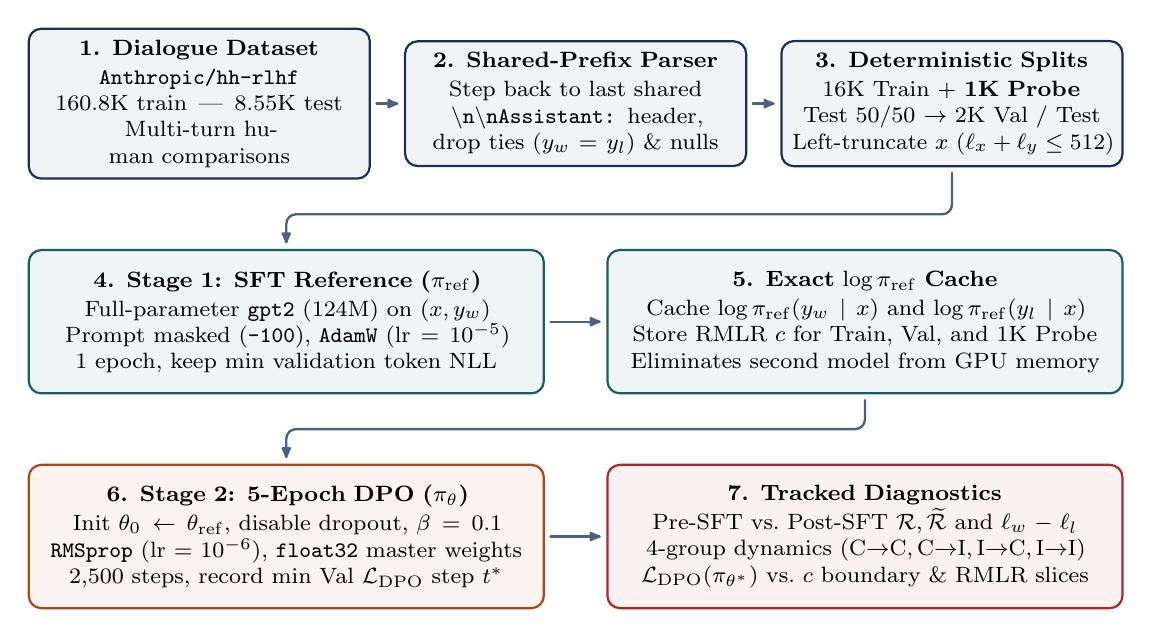
\begin{tikzpicture}[
    box/.style={
      rectangle, rounded corners=4.5pt, draw=#1!85!black, line width=0.8pt,
      fill=#1!6, text width=4.05cm, minimum height=1.54cm,
      align=center, font=\footnotesize, inner sep=4pt
    },
    widebox/.style={
      rectangle, rounded corners=4.5pt, draw=#1!85!black, line width=0.8pt,
      fill=#1!7, text width=6.26cm, minimum height=1.82cm,
      align=center, font=\footnotesize, inner sep=4pt
    },
    arrow/.style={
      -{Latex[length=1.85mm, width=1.45mm, round]},
      line width=0.85pt,
      draw=navybox!80,
      line cap=round,
      line join=round,
      shorten <=2.0pt,
      shorten >=2.0pt
    }
  ]
    % Row 1: Three equal-height data preparation boxes
    \node[box=navybox] (raw) {
      \textbf{1. Dialogue Dataset}\\[1pt]
      \texttt{Anthropic/hh-rlhf}\\
      160.8K train \,|\, 8.55K test\\
      Multi-turn human comparisons
    };

    \node[box=navybox, right=0.42cm of raw] (parse) {
      \textbf{2. Shared-Prefix Parser}\\[1pt]
      Step back to last shared\\
      \texttt{\textbackslash n\textbackslash nAssistant:} header,\\
      drop ties ($y_w = y_l$) \& nulls
    };

    \node[box=navybox, right=0.42cm of parse] (splits) {
      \textbf{3. Deterministic Splits}\\[1pt]
      16K Train + \textbf{1K Probe}\\
      Test $50/50 \to$ 2K Val / Test\\
      Left-truncate $x$ ($\ell_x + \ell_y \le 512$)
    };

    % Row 2: Two equal-height Stage 1 & Cache boxes aligned horizontally
    \node[widebox=tealbox, below=0.88cm of raw.south west, anchor=north west] (sft) {
      \textbf{4. Stage 1: SFT Reference ($\piref$)}\\[1pt]
      Full-parameter \texttt{gpt2} (124M) on $(x, y_w)$\\
      Prompt masked (\texttt{-100}), \texttt{AdamW} ($\text{lr}=10^{-5}$)\\
      1 epoch, keep min validation token NLL
    };

    \node[widebox=tealbox, at=(sft.north -| splits.east), anchor=north east] (cache) {
      \textbf{5. Exact $\log \piref$ Cache}\\[1pt]
      Cache $\log \piref(y_w \mid x)$ and $\log \piref(y_l \mid x)$\\
      Store RMLR $c$ for Train, Val, and 1K Probe\\
      Eliminates second model from GPU memory
    };

    % Row 3: Two equal-height Stage 2 & Diagnostics boxes aligned horizontally
    \node[widebox=amberbox, below=0.88cm of sft.south west, anchor=north west] (dpo) {
      \textbf{6. Stage 2: 5-Epoch DPO ($\pitheta$)}\\[1pt]
      Init $\theta_0 \leftarrow \theta_{\mathrm{ref}}$, disable dropout, $\beta = 0.1$\\
      \texttt{RMSprop} ($\text{lr}=10^{-6}$), \texttt{float32} master weights\\
      2,500 steps, record min Val $\LDPO$ step $t^*$
    };

    \node[widebox=crimson, at=(dpo.north -| splits.east), anchor=north east] (eval) {
      \textbf{7. Tracked Diagnostics}\\[1pt]
      Pre-SFT vs.\ Post-SFT $\Racc, \Racctilde$ and $\ell_w - \ell_l$\\
      4-group dynamics ($\CtoC, \CtoI, \ItoC, \ItoI$)\\
      $\LDPO(\pithetastar)$ vs.\ $c$ boundary \& RMLR slices
    };

    % Smooth, exact 4-point midpoint corridors (zero overshoot, rounded bends)
    \coordinate (mid12) at ($(raw.south)!0.5!(sft.north)$);
    \coordinate (mid23) at ($(sft.south)!0.5!(dpo.north)$);

    \draw[arrow] (raw.east) -- (parse.west);
    \draw[arrow] (parse.east) -- (splits.west);
    \draw[arrow, rounded corners=3.5pt]
      (splits.south) -- (splits.south |- mid12) -- (sft.north |- mid12) -- (sft.north);
    \draw[arrow] (sft.east) -- (cache.west);
    \draw[arrow, rounded corners=3.5pt]
      (cache.south) -- (cache.south |- mid23) -- (dpo.north |- mid23) -- (dpo.north);
    \draw[arrow] (dpo.east) -- (eval.west);
  \end{tikzpicture}
  \caption{\textbf{Seven-Stage \texttt{GPT-2} (124M) SFT-to-DPO Pipeline} (\prefnb{} \,\textbullet\, \ghrepo{}).}
  \label{fig:pipeline_schematic}
\end{figure}

Figure~\ref{fig:pipeline_schematic} summarizes our end-to-end PyTorch pipeline in \prefnb{}, trained on Anthropic's helpfulness and harmlessness dialogue dataset \citep[\texttt{Anthropic/hh-rlhf},][]{bai2022training}. Under a single-GPU compute budget, we train full-parameter \texttt{gpt2} ($124$M) on $16{,}000$ pairs instead of Chen et al.'s multi-GPU $160$K-pair runs on larger models ($1{,}000$-pair training probe and $2{,}000$-pair validation split from the deterministic \texttt{seed=0} $50/50$ test split). Stage~1 runs $1$ epoch of SFT ($500$ steps, batch size $32$) on $(x, y_w)$ with \texttt{AdamW} ($\text{lr} = 10^{-5}$). Stage~2 initializes $\theta_0 \leftarrow \theta_{\mathrm{ref}}$, disables all $37$ \texttt{nn.Dropout} modules in \texttt{gpt2} (matching \texttt{dpo\_trainer.py}, line~373, so \texttt{train()}-mode policy log-probabilities match cached \texttt{eval()}-mode $\log \piref$ at Step~$0$), and runs $5$ epochs of DPO ($2{,}500$ steps, $\beta = 0.1$, gradient clipping at $1.0$, linear warmup and decay) with \texttt{RMSprop} ($\alpha = 0.99$, $\epsilon = 10^{-8}$).

\subsection{Official Codebase Audit Versus Our Implementation}

\begin{table}[t]
  \centering
  \caption{\textbf{Implementation Errors Identified in the Official Repository (\officialreposhort{}) of \citet{chen2024preference} Versus Our Fixes in \prefnb{} / \ghrepo{}.}}
  \label{tab:codebase_vs_ours}
  \footnotesize
  \renewcommand{\arraystretch}{1.16}
  \setlength{\tabcolsep}{3.5pt}
  \begin{tabular*}{\textwidth}{@{\extracolsep{\fill}}>{\raggedright\arraybackslash}p{4.05cm} >{\raggedright\arraybackslash}p{4.65cm} >{\raggedright\arraybackslash}p{4.45cm}@{}}
    \toprule
    \textbf{Official Script \& Location} & \textbf{Bug in Official Code} & \textbf{Our Fix in \prefnb{}} \\
    \midrule
    \textbf{1.\ Idealized $\Racc^*$ Ratio}\newline {\scriptsize\texttt{rlhf\_minimizer\_client.py}} (L215--218) & Divides negative log-probs $(-L_1)/(-L_2) = L_1/L_2$ without \texttt{np.exp} when \texttt{normalized=False}, inverting length penalties and inflating $\Racc^*$. & Evaluates all ranking conditions directly in log-probability space ($\delta_\theta \ge 0$ and $\frac{1}{\beta}\log\frac{p}{1-p} > c$). \\
    \addlinespace[2.5pt]
    \textbf{2.\ Observed $\Racc$ Overflow}\newline {\scriptsize\texttt{calibration\_metrics\_lib.py}} (L166--195) & Computes \texttt{np.exp(log\_p1 - log\_p2)} in \texttt{float64}, overflowing to \texttt{+inf} when $\delta_\theta > 709.78$ and dropping strongly correct pairs via \texttt{\textasciitilde np.isinf}. & Compares \texttt{logp\_yw >= logp\_yl} directly without exponentiation, retaining $100\%$ of pairs across $c \in [-700.64, +724.72]$. \\
    \addlinespace[2.5pt]
    \textbf{3.\ Dialogue Slicing \& BPE}\newline {\scriptsize\texttt{process\_rlhf\_datasets.py}} (L77--81), {\scriptsize\texttt{perplexity\_lib.py}} (L48--84) & Slices {\scriptsize\texttt{rejected[len(prompt):]}} at \texttt{chosen}'s index, keeps exact ties, and right-truncates {\scriptsize\texttt{f"\{input\} \{output\}"}}, causing BPE drift and $0/0$ \texttt{NaN}s on long prompts. & Backtracks to last shared \texttt{\textbackslash n\textbackslash nAssistant:} turn, drops $922$ train / $47$ test tied or empty rows, tokenizes $x$ and $y$ separately, and left-truncates $x$. \\
    \addlinespace[2.5pt]
    \textbf{4.\ Tail Loss Rounding}\newline {\scriptsize\texttt{dpo\_trainer.py}} (L1065) & Evaluates {\scriptsize\texttt{-F.logsigmoid(beta*logits)}} in \texttt{float32}, rounding $1 + e^{-u}$ to $1.0$ ($\LDPO = 0$) for $c \ge 167$ ($85.1\%$ false tail flips). & Uses piecewise {\scriptsize\texttt{neg\_logsigmoid\_exact}} in \texttt{float64} ($0\%$ false flips up to $c \approx 7{,}090$, exact $-0.5$ Step-$0$ gradient). \\
    \bottomrule
  \end{tabular*}
\end{table}

Auditing every script in the official repository revealed four concrete bugs summarized in Table~\ref{tab:codebase_vs_ours}. Beyond the missing \texttt{np.exp} in \texttt{rlhf\_minimizer\_client.py} (\S\ref{sec:critique}), \texttt{calibration\_metrics\_lib.py} exponentiates $\delta_\theta$ in \texttt{float64} and filters out \texttt{inf}: strongly correct pairs ($\delta_\theta > 709.78$) overflow to \texttt{+inf} and are discarded, whereas strongly misranked pairs ($\delta_\theta < -709.78$, such as our probe extreme at $c = +724.72$) underflow to \texttt{0.0} and remain in the denominator, biasing observed $\Racc$ downward. Similarly, \texttt{process\_rlhf\_datasets.py} slices \texttt{rejected} using the character offset of \texttt{chosen}'s final turn (cutting mid-turn whenever dialogues diverge earlier) and keeps exact ties, while \texttt{perplexity\_lib.py} right-truncates concatenated text at $512$ tokens (deleting the entire response on long prompts). Our parser backtracks from the first character divergence to the last shared \texttt{\textbackslash n\textbackslash nAssistant:} header, removes $740$ identical ties and $182$ empty/tied continuations in train ($159{,}878$ clean pairs) plus $47$ in test ($8{,}505$ clean pairs), prepends \texttt{bos\_token\_id}, tokenizes $x$ and space-prefixed $y$ separately, caps $\ell_y \le 256$, and left-truncates $x$ within $512$ tokens.

\subsection{Response-Length Dispersion Across 16,000 Dialogue Pairs}

\begin{table}[t]
  \centering
  \caption{\textbf{Word-Length Distribution Across $16{,}000$ Cleaned Training Pairs} (Cell~4 of \prefnb{}). Preferred replies $y_w$ are longer than $y_l$ in $51.0\%$ of pairs, with a wide upper tail.}
  \label{tab:hh_eda_lengths}
  \small
  \setlength{\tabcolsep}{4.8pt}
  \begin{tabular*}{\textwidth}{@{\extracolsep{\fill}}lcccccccc@{}}
    \toprule
    \textbf{Quantity (words)} & \textbf{Mean} & \textbf{Std} & \textbf{Min} & \textbf{25\%} & \textbf{50\%} & \textbf{75\%} & \textbf{95\%} & \textbf{Max} \\
    \midrule
    Prompt $x$ & 110.9 & 121.1 & 3 & 19 & 75 & 158 & 334 & 1,473 \\
    Preferred reply $y_w$ & 55.3 & 52.0 & 1 & 18 & 39 & 77 & 165 & 791 \\
    Dispreferred reply $y_l$ & 52.6 & 51.5 & 1 & 16 & 36 & 72 & 166 & 639 \\
    \textbf{Length gap ($y_w$ minus $y_l$)} & \textbf{+2.6} & \textbf{51.9} & $\boldsymbol{-410}$ & $\boldsymbol{-19}$ & \textbf{+1} & \textbf{+24} & \textbf{+86} & \textbf{+622} \\
    \bottomrule
  \end{tabular*}
\end{table}

\begin{figure}[t]
  \centering
  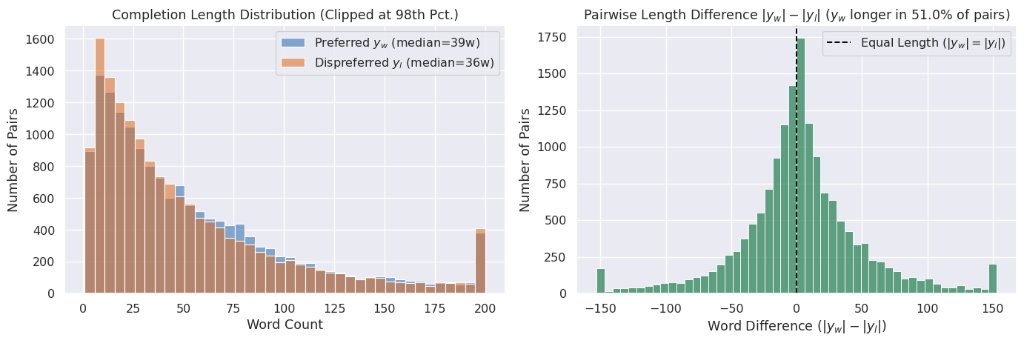
\includegraphics[width=\textwidth]{dpo_ranking_replication_outputs/eda_hh_rlhf_lengths.png}
  \caption{\textbf{Completion Length Distributions Across $16{,}000$ Cleaned Training Pairs} (\prefnb{}). \textbf{Left:} Word counts of $y_w$ (median $39$w) and $y_l$ (median $36$w), clipped at the $98$th percentile. \textbf{Right:} Pairwise word-count difference ($\text{std} = 51.9$ words, $95$th percentile $+86$ words).}
  \label{fig:hh_eda_lengths}
\end{figure}

Table~\ref{tab:hh_eda_lengths} and Figure~\ref{fig:hh_eda_lengths} show why SFT policies exhibit heavy positive $c$ tails. Although the median length gap between $y_w$ and $y_l$ is only $+1$ word (mean $+2.6$ words), the pairwise standard deviation is $51.9$ words, reaching $+86$ words at the $95$th percentile and $+622$ words maximum. Because each extra token contributes roughly $2.4$ nats of negative log-likelihood under \texttt{GPT-2}, pairs in the top $5\%$ penalize $\log \piref(y_w \mid x)$ by more than $250$ nats relative to $y_l$ \citep{singhal2023long}, generating $c > 100$ even when per-token likelihoods are equal. Prompts also exceed $334$ words on $5\%$ of dialogues (up to $1{,}473$ words), confirming why left-truncating $x$ rather than right-truncating $(x, y)$ is essential.

% =========================================================================
\section{Floating-Point and Mixed-Precision Findings}
\label{sec:numerical}
% =========================================================================

While implementing and running \prefnb{}, we encountered two distinct floating-point bugs that silently corrupt Theorem~\ref{thm:flip_threshold} verification and mixed-precision DPO optimization.

\subsection{Tail \texttt{log1p} Truncation and Step-0 Subgradients}

\begin{figure}[t]
  \centering
  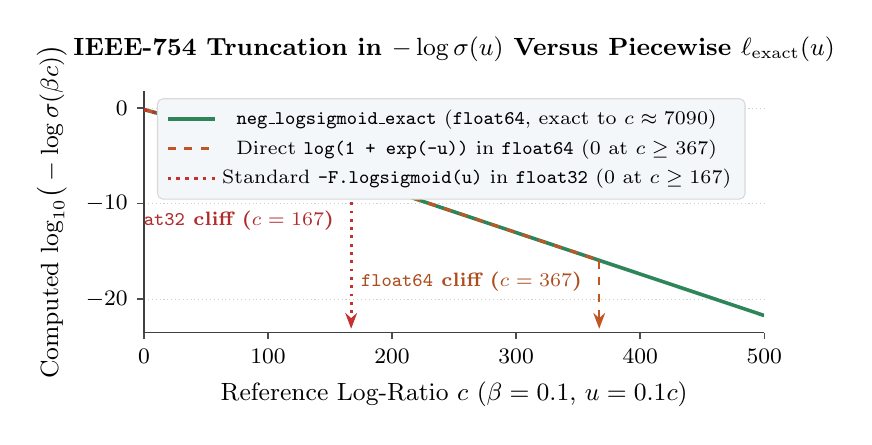
\begin{tikzpicture}
    \begin{axis}[
      neuripsplot,
      width=0.78\textwidth,
      height=4.65cm,
      xlabel={Reference Log-Ratio $c$ ($\beta = 0.1$, $u = 0.1c$)},
      ylabel={Computed $\log_{10}\!\big(-\log\sigma(\beta c)\big)$},
      xmin=0, xmax=500,
      ymin=-23.5, ymax=1.8,
      title={IEEE-754 Truncation in $-\log\sigma(u)$ Versus Piecewise $\ell_{\mathrm{exact}}(u)$},
      legend pos=north east,
      legend style={font=\scriptsize, fill=slatefill!70, draw=gray!30, rounded corners=2pt}
    ]
      \addplot[line width=1.3pt, forest, samples=150, domain=0:500]
        {ifthenelse(0.1*x < 5, log10(ln(1 + exp(-min(0.1*x, 5)))), -0.1*x*0.43429448)};
      \addlegendentry{\texttt{neg\_logsigmoid\_exact} (\texttt{float64}, exact to $c \approx 7090$)}

      \addplot[line width=1.05pt, amberbox, dashed, samples=120, domain=0:366]
        {ifthenelse(0.1*x < 5, log10(ln(1 + exp(-min(0.1*x, 5)))), -0.1*x*0.43429448)};
      \addlegendentry{Direct \texttt{log(1 + exp(-u))} in \texttt{float64} ($0$ at $c \ge 367$)}
      \draw[line width=0.9pt, amberbox, dashed, -{Stealth[length=2.0mm]}] (axis cs:367,-15.94) -- (axis cs:367,-23.1);

      \addplot[line width=1.2pt, crimson, dotted, samples=90, domain=0:166]
        {ifthenelse(0.1*x < 5, log10(ln(1 + exp(-min(0.1*x, 5)))), -0.1*x*0.43429448)};
      \addlegendentry{Standard \texttt{-F.logsigmoid(u)} in \texttt{float32} ($0$ at $c \ge 167$)}
      \draw[line width=1.0pt, crimson, dotted, -{Stealth[length=2.0mm]}] (axis cs:167,-7.25) -- (axis cs:167,-23.1);

      \node[font=\scriptsize\bfseries, text=crimson!90!black, anchor=east] at (axis cs:161,-11.8)
        {\texttt{float32} cliff ($c = 167$)};
      \node[font=\scriptsize\bfseries, text=amberbox!90!black, anchor=east] at (axis cs:361,-18.2)
        {\texttt{float64} cliff ($c = 367$)};
      \filldraw[royalblue] (axis cs:176.45,-7.665) circle (2.0pt);
      \node[font=\scriptsize, text=royalblue!90!black, anchor=south west] at (axis cs:182,-7.3)
        {Hard-slice med.\ ($c=176.5$)};
    \end{axis}
  \end{tikzpicture}
  \caption{\textbf{IEEE-754 Precision Cliffs in $-\log\sigma(u)$.} Once $e^{-u} < \varepsilon_{\mathrm{mach}}/2$, $1.0 + e^{-u}$ rounds to $1.0$, collapsing both $\LDPO$ and $f(c)$ to $0$ just below our hard-slice median $c = 176.5$ in \texttt{float32} and well below our probe maximum $c = 724.7$ in \texttt{float64}.}
  \label{fig:numerical_cliff}
\end{figure}

\begin{table}[t]
  \centering
  \caption{\textbf{IEEE-754 Tail Precision and Step-0 Subgradient Audit} across $N = 10{,}000$ wide-tail pairs ($4{,}977$ misranked pairs with $\delta_\theta < 0$, including $375$ at $c \ge 167$ and $108$ at $c \ge 367$, Cell~5 of \prefnb{}).}
  \label{tab:precision_audit}
  \footnotesize
  \setlength{\tabcolsep}{2.4pt}
  \begin{tabular*}{\textwidth}{@{\extracolsep{\fill}}lcccc@{}}
    \toprule
    \textbf{Loss Formula} & \textbf{Precision} & \textbf{False Flips} & \textbf{Tail Error Rate} & \textbf{Step-0 $\nabla_u \ell(0)$} \\
    \midrule
    \texttt{-F.logsigmoid(u)} ($\LDPO \le f(c)$) & \texttt{float32} & 324 / 4,977 & 85.1\% ($c \ge 167$) & $-0.5$ (Exact) \\
    \texttt{-F.logsigmoid(u)} + $10^{-6}$ slack & \texttt{float32} & 399 / 4,977 & 100.0\% ($c \ge 167$) & $-0.5$ (Exact) \\
    Direct \texttt{log(1 + exp(-u))} & \texttt{float64} & 91 / 4,977 & 82.4\% ($c \ge 367$) & $-0.5$ (Exact) \\
    \texttt{clamp(-u,0)+log1p(exp(-|u|))} & \texttt{float64} & 0 / 4,977 & 0.0\% & $-1$ / $0$ (\textbf{Broken}) \\
    \textbf{Piecewise $\ell_{\mathrm{exact}}(u)$ (Eq.~\ref{eq:hybrid_loss})} & \texttt{float64} & \textbf{0 / 4,977} & \textbf{0.0\%} & $\boldsymbol{-0.5}$ \textbf{(Exact)} \\
    \bottomrule
  \end{tabular*}
\end{table}

PyTorch's \texttt{F.softplus(-u, threshold=20)} and \texttt{-F.logsigmoid(u)} (\texttt{dpo\_trainer.py}, line~1065) switch to a linear branch only for $u < -20$. For $u > 0$, they form $1.0 + e^{-u}$ explicitly, rounding to $1.0$ and returning $0.0$ whenever $e^{-u} < \varepsilon_{\mathrm{mach}}/2$ ($c \ge 167$ in \texttt{float32} and $c \ge 367$ in \texttt{float64}, Figure~\ref{fig:numerical_cliff}). In our $10{,}000$-pair audit (Table~\ref{tab:precision_audit}), \texttt{float32} evaluation falsely marks $85.1\%$ of misranked pairs with $c \ge 167$ as flipped ($\LDPO = 0 \le 0 = f(c)$). Conversely, replacing $-\log\sigma(u)$ with $\operatorname{clamp}(-u, \min=0) + \operatorname{log1p}(e^{-|u|})$ (\texttt{dpo\_trainer.py}, line~675) corrupts Step-$0$ gradients: at $u = 0$, PyTorch autograd evaluates the kink subgradient as $-1.0$ (or $0.0$ under \texttt{relu}) instead of $-\sigma(0) = -0.5$. Splitting the domain away from $u = 0$ at $u = 10$ resolves both problems:
\begin{equation}
  \ell_{\mathrm{exact}}(u) =
  \begin{cases}
    -\operatorname{logsigmoid}(u), & u \le 10, \\[2pt]
    \operatorname{log1p}\!\big(\exp(-\max(u, 10))\big), & u > 10,
  \end{cases}
  \label{eq:hybrid_loss}
\end{equation}
preserving exact C++ \texttt{logsigmoid} gradients for all $u \le 10$ and full mantissa accuracy up to $c \approx 7{,}090$.

\subsection{Master-Weight Rounding Under \texttt{bfloat16} Versus \texttt{float32}}

Our initial \texttt{GPT-2} run on an \texttt{NVIDIA L4} GPU ($22$\,GB VRAM) uncovered a second precision trap when trainable parameters are stored directly in \texttt{bfloat16}. Although \texttt{bfloat16} preserves the $8$-bit exponent range of \texttt{float32} (preventing underflow in $\epsilon = 10^{-8}$), it retains only $7$ fraction bits ($\varepsilon_{\mathrm{bf16}} = 2^{-7} \approx 7.81 \times 10^{-3}$). Near a typical weight magnitude $|w| \approx 0.1$, half a unit in the last place is $2^{-4} \times 2^{-8} \approx 2.44 \times 10^{-4}$. Under \texttt{RMSprop} at $\text{lr} = 10^{-6}$, each normalized update $-\eta \, g / \sqrt{v} \approx 10^{-6}$ is $244\times$ smaller than $0.5\text{ ULP}$, so IEEE-754 round-to-nearest-even maps $w - \eta \, g / \sqrt{v} \mapsto w$ and freezes $\LDPO$ at $\ln 2 = 0.6931$ ($t^* = 0$, $0.93\%$ flipped across $5$ epochs). Keeping trainable master weights in \texttt{float32} ($23$ fraction bits, $\varepsilon_{\mathrm{fp32}} = 1.19 \times 10^{-7}$) while running forward passes under \texttt{bfloat16} \texttt{autocast} resolves every update cleanly.

% =========================================================================
\section{Empirical Observations and Results}
\label{sec:results}
% =========================================================================

\begin{figure}[t]
  \centering
  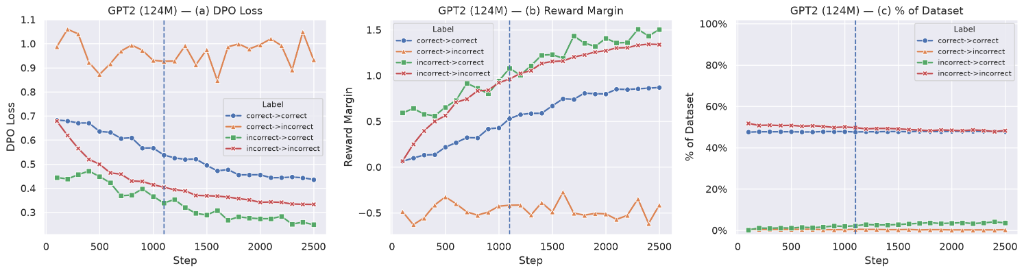
\includegraphics[width=\textwidth]{dpo_ranking_replication_outputs/figure2_dpo_dynamics.png}
  \caption{\textbf{5-Epoch \texttt{GPT-2} (124M) DPO Training Dynamics on an \texttt{NVIDIA A100 80GB} GPU} ($16{,}000$ training pairs, $2{,}500$ steps, $1{,}000$-pair probe in \prefnb{}, dashed vertical line at lowest validation loss step $t^* = 1{,}100$). \textbf{(a)} Mean $\LDPO$ drops continuously across both $\CtoC$ and $\ItoI$. \textbf{(b)} Mean margin $\bar{u}_\theta$ climbs steadily across all optimized groups. \textbf{(c)} Only $4.24\%$ ($22/519$) of initially misranked pairs transition into $\ItoC$ by $t^*$ ($6.94\%$ by Step~$2{,}500$).}
  \label{fig:gpt2_a100_dynamics}
\end{figure}

\begin{figure}[t]
  \centering
  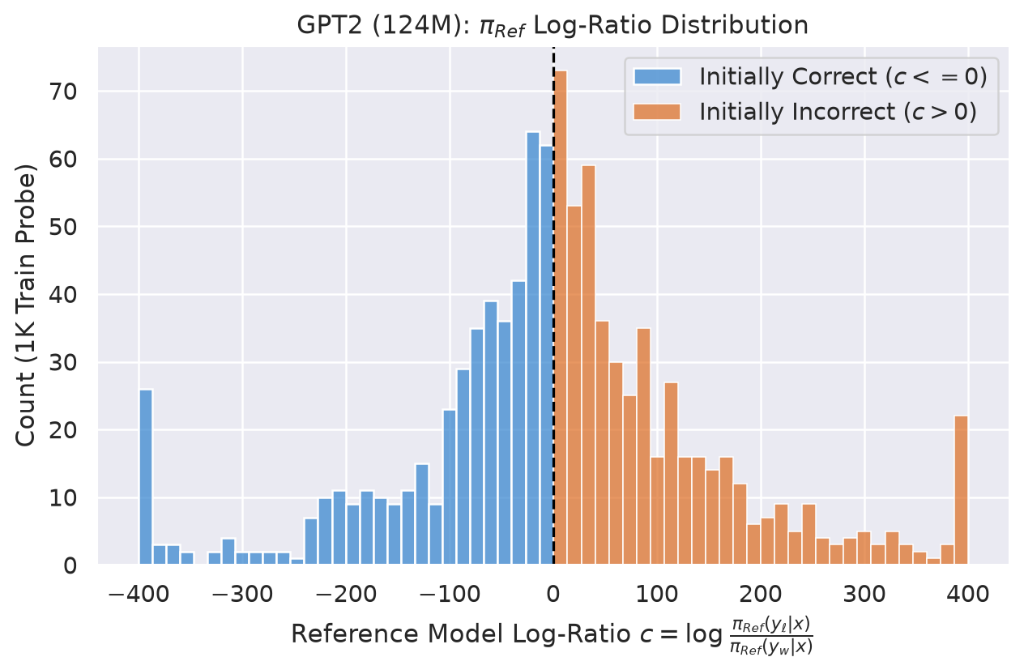
\includegraphics[height=4.85cm,keepaspectratio]{dpo_ranking_replication_outputs/rmlr_distribution_gpt2.png}\hfill
  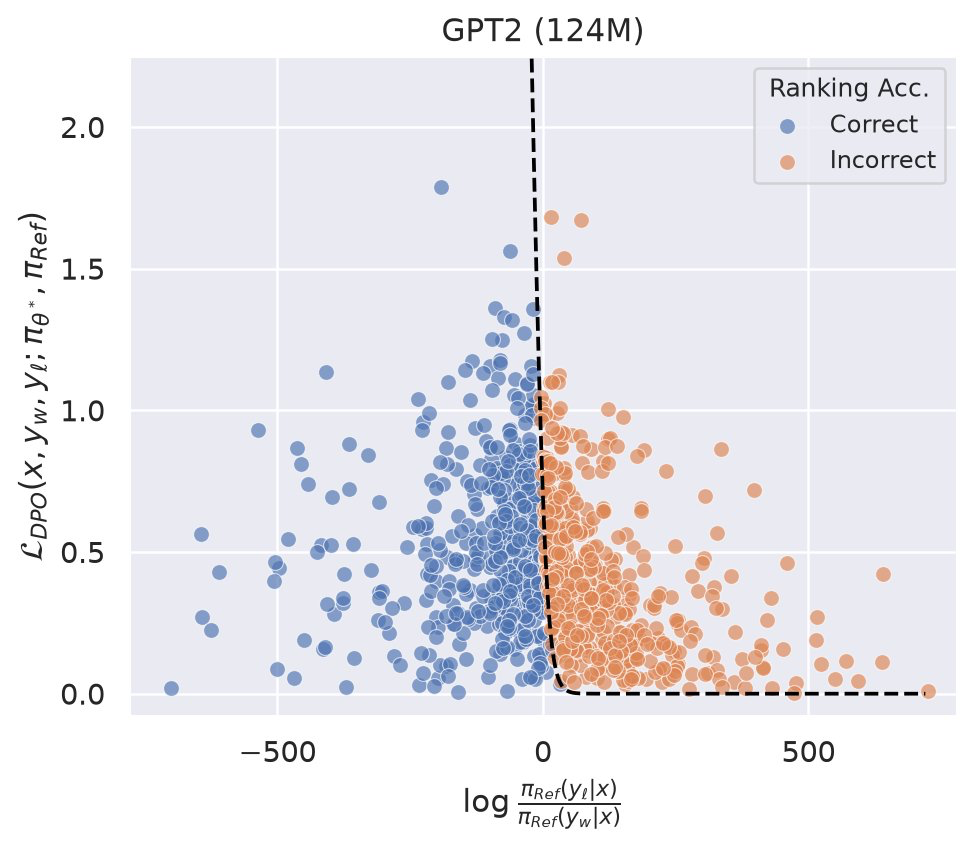
\includegraphics[height=4.85cm,keepaspectratio]{dpo_ranking_replication_outputs/figure3_theorem4_1_boundary.png}
  \caption{\textbf{Reference Conditioning and Phase-Boundary Verification on $1{,}000$ Probe Pairs} (\texttt{GPT-2} 124M, \prefnb{}). \textbf{Left:} Post-SFT $\piref$ RMLR distribution ($48.1\%$ with $c \le 0$ and $51.9\%$ with $c > 0$, including $30.7\%$ at $c > 50$). \textbf{Right:} Per-pair $\LDPO(\pithetastar)$ at $t^* = 1{,}100$ versus $c \in [-700.64, +724.72]$, matching the dashed Theorem~\ref{thm:flip_threshold} boundary $f(c) = -\log\sigma(\beta c)$ on $1{,}000/1{,}000$ pairs ($100.0\%$).}
  \label{fig:gpt2_rmlr_and_boundary}
\end{figure}

\begin{table}[t]
  \centering
  \caption{\textbf{End-to-End \texttt{GPT-2} (124M) Stage Progression and Four-Group DPO Decomposition} on our \texttt{NVIDIA A100 80GB} run ($16{,}000$ train pairs, $1{,}000$-pair probe, $2{,}000$-pair validation split, $95\%$ bootstrap CI $[46.2\%, 50.7\%]$ on Val $\Racc$ at $t^*$). For reference, \citet{chen2024preference} report pretrained \texttt{GPT-2} $\Racc / \Racctilde = 46.8\% / 52.7\%$ on train and $46.0\% / 49.9\%$ on test.}
  \label{tab:gpt2_progression}
  \footnotesize
  \setlength{\tabcolsep}{1.8pt}
  \begin{tabular*}{\textwidth}{@{\extracolsep{\fill}}lccccc@{}}
    \toprule
    \textbf{Stage / Group} & \textbf{Probe $\LDPO$} & \textbf{Mean $\bar{u}_\theta$} & \textbf{Probe $\Racc / \Racctilde$} & \textbf{Val $\Racc / \Racctilde$} & \textbf{Flip / Transition} \\
    \midrule
    Pretrained (Pre-SFT) & N/A & N/A & 46.6\% / 53.6\% & N/A & N/A \\
    SFT ($\piref$, Step 0) & $0.6931$ & $+0.000$ & 48.1\% / 55.1\% & 48.2\% / 52.2\% & 0/519 (0.0\%) \\
    \textbf{DPO ($\pithetastar$, $t^*\!=\!1100$)} & $\boldsymbol{0.4690}$ & $\boldsymbol{+0.751}$ & \textbf{49.8\% / 62.7\%} & \textbf{48.5\% / 55.5\%} & \textbf{22/519 (4.24\%)} \\
    DPO (Ep.\ 5, $t\!=\!2500$) & $0.3807$ & $+1.115$ & 51.4\% / 65.6\% & Overfit & 36/519 (6.94\%) \\
    \midrule
    \multicolumn{6}{@{}l}{\emph{Four-Group Probe Trajectory ($t^* = 1{,}100 \longrightarrow$ Epoch 5, Step $2{,}500$):}} \\[1.5pt]
    \quad $\CtoC$ (Kept correct) & $0.538\!\to\!0.436$ & $+0.53\!\to\!+0.87$ & \multicolumn{2}{c}{47.6\% $\to$ 47.8\% of probe} & 99.0\% $\to$ 99.4\% \\
    \quad $\CtoI$ (Lost correct) & $0.927\!\to\!0.934$ & $-0.42\!\to\!-0.42$ & \multicolumn{2}{c}{0.5\% $\to$ 0.3\% of probe} & 1.0\% $\to$ 0.6\% \\
    \quad $\ItoC$ (Flipped wrong) & $0.339\!\to\!0.249$ & $+1.08\!\to\!+1.51$ & \multicolumn{2}{c}{2.2\% $\to$ 3.6\% of probe} & \textbf{4.24\% $\to$ 6.94\%} \\
    \quad $\ItoI$ (Stuck wrong) & $0.404\!\to\!0.333$ & $+0.96\!\to\!+1.34$ & \multicolumn{2}{c}{49.7\% $\to$ 48.3\% of probe} & 95.8\% $\to$ 93.1\% \\
    \bottomrule
  \end{tabular*}
\end{table}

\begin{table}[t]
  \centering
  \caption{\textbf{RMLR Regime Breakdown and the Hard-Tail Loss Paradox on $1{,}000$ Probe Pairs} (\texttt{GPT-2} 124M at $t^* = 1{,}100$). Across all $519$ misranked pairs ($c > 0$), the median required flip loss is $0.0008$.}
  \label{tab:gpt2_probe_slices}
  \footnotesize
  \setlength{\tabcolsep}{2.0pt}
  \begin{tabular*}{\textwidth}{@{\extracolsep{\fill}}lcccccc@{}}
    \toprule
    \textbf{$\piref$ RMLR Regime} & \textbf{Share} & \textbf{Med.\ $c$} & \textbf{$\ell_w / \ell_l$ (tok)} & \textbf{Med.\ $\LDPO$} & \textbf{Req.\ $f(\text{med }c)$} & \textbf{Flip $t^* / \text{Ep5}$} \\
    \midrule
    Easy-to-Learn ($c < -50$) & 28.3\% & $-121.81$ & 60.6 / 122.2 & $0.485$ & $12.18$ & N/A ($c < 0$) \\
    Easy-to-Flip ($0 < c \le 2$) & 1.3\% & $+1.17$ & 56.5 / 52.9 & $0.602$ & $0.636$ & \textbf{53.8\% / 69.2\%} \\
    Intermediate & 50.2\% & $+13.07$ & 52.6 / 45.2 & $0.469$ & $0.239$ & 3.0\% / 5.4\% \\
    \textbf{Hard-to-Learn ($c > 100$)} & \textbf{20.2\%} & $\boldsymbol{+176.45}$ & \textbf{146.0 / 58.4} & $\boldsymbol{0.217}$ & $\boldsymbol{2.16 \times 10^{-8}}$ & \textbf{0.0\% / 0.0\%} \\
    \bottomrule
  \end{tabular*}
\end{table}

Figures~\ref{fig:gpt2_a100_dynamics} and~\ref{fig:gpt2_rmlr_and_boundary} and Tables~\ref{tab:gpt2_progression} and~\ref{tab:gpt2_probe_slices} present our complete \texttt{float32}-master-weight \texttt{GPT-2} (124M) experimental results on an \texttt{NVIDIA A100 80GB} GPU. Four clear empirical observations emerge:

\begin{enumerate}[leftmargin=1.8em,itemsep=2.5pt,topsep=2pt]
  \item \textbf{SFT Lowers Perplexity Without Teaching Pairwise Ranking (Claim~1):} Raw pretrained \texttt{GPT-2} achieves $\Racc = 46.6\%$ and $\Racctilde = 53.6\%$ on the $1{,}000$-pair probe, closely matching Chen et al.'s reported $46.8\% / 52.7\%$. Fine-tuning on preferred replies $(x, y_w)$ reduces validation token NLL to $2.3635$, yet lifts probe ranking accuracy by only $+1.5$\,pp to $\Racc(\piref) = 48.1\%$ ($48.2\%$ on validation). Because cross-entropy SFT never sees $y_l$, $519$ of $1{,}000$ pairs ($51.9\%$) enter DPO misranked ($c > 0$), including $30.7\%$ above $c = 50$ ($f(50) = 0.0067$) and $20.2\%$ above $c = 100$ (Figure~\ref{fig:gpt2_rmlr_and_boundary}, left).

  \item \textbf{DPO Reduces Loss by $45\%$ While Flipping Only $4.24\%$ of Misranked Pairs at $t^*$ (Claim~3):} Across $2{,}500$ steps in Figure~\ref{fig:gpt2_a100_dynamics} and Table~\ref{tab:gpt2_progression}, mean probe $\LDPO$ falls steadily from $0.6931$ at Step~$0$ to $0.4690$ at $t^* = 1{,}100$ ($-32.3\%$) and $0.3807$ at Epoch~$5$ ($-45.1\%$), while mean margin $\bar{u}_\theta$ climbs from $0$ to $+0.751$ and $+1.115$. Despite this substantial loss reduction, only $22$ of $519$ misranked pairs ($4.24\% < 10\%$) flip into $\ItoC$ at $t^* = 1{,}100$, rising to only $36 / 519$ ($6.94\%$) even after $5$ full epochs. Raw accuracy $\Racc$ gains just $+1.7$\,pp on the probe at $t^*$ ($48.1\% \to 49.8\%$) and $+0.3$\,pp on validation ($48.2\% \to 48.5\%$, $95\%$ bootstrap CI $[46.2\%, 50.7\%]$).

  \item \textbf{Length Normalization Recovers $+7.6$\,pp Masked by Sequence Length:} While raw probe $\Racc$ barely moves ($+1.7$\,pp at $t^*$), length-normalized probe accuracy $\Racctilde$ rises by $+7.6$\,pp at $t^*$ ($55.1\% \to 62.7\%$) and $+10.5$\,pp by Epoch~$5$ ($65.6\%$). DPO therefore increases per-token log-probability on $y_w$ relative to $y_l$, but whenever $\ell_w \gg \ell_l$, summing over $\ell_w$ tokens keeps total $\delta_\theta < 0$.

  \item \textbf{The Hard-Tail Loss Paradox ($0.217$ Median Loss Yet $0.0\%$ Flips, Claim~4):} In Figure~\ref{fig:gpt2_rmlr_and_boundary} (right), every single probe pair ($1{,}000 / 1{,}000$, $100.0\%$) obeys $\delta_{\theta^*} \ge 0 \iff \LDPO(\pithetastar) \le f(c)$. Comparing slices in Table~\ref{tab:gpt2_probe_slices} uncovers a striking pattern that also explains why the red $\ItoI$ loss curve ($0.404$) lies \emph{below} the blue $\CtoC$ curve ($0.538$) in Figure~\ref{fig:gpt2_a100_dynamics}(a). On Hard-to-Learn pairs ($c > 100$, $n = 202$), preferred replies average $\ell_w = 146.0$ tokens versus $\ell_l = 58.4$ tokens ($2.5\times$ longer). Because a small per-token probability gain summed across $146$ tokens produces a large positive shift in $\delta_\theta - \delta_{\theta_0} = \delta_\theta + c$, $u_\theta = \beta(\delta_\theta + c)$ grows rapidly and drives median $\LDPO(t^*)$ down to $0.217$, the \emph{lowest} loss of all four regimes. Yet because $\delta_{\theta_0} = -c \approx -176.5$, gaining $+15\text{--}20$ nats still leaves $\delta_{\theta^*} \approx -158 \ll 0$ ($0.217 \gg f(176.45) = 2.16 \times 10^{-8}$), resulting in $0.0\%$ flips ($0 / 202$) at both $t^*$ and Epoch~$5$. By contrast, in the narrow Easy-to-Flip band ($0 < c \le 2$, $n = 13$, $\ell_w / \ell_l = 56.5 / 52.9$ tokens), a modest median loss of $0.602 \le f(1.17) = 0.636$ flips $53.8\%$ of pairs at $t^*$ and $69.2\%$ by Epoch~$5$.
\end{enumerate}

% =========================================================================
\section{Conclusion and Implications for Alignment Objectives}
\label{sec:discussion}
% =========================================================================

Our theoretical analysis, codebase audit, and 5-epoch \texttt{GPT-2} experiments give a complete picture of why DPO minimizes training loss without learning pairwise preference rankings. After correcting four implementation bugs in the official scripts (Table~\ref{tab:codebase_vs_ours}) and two floating-point pitfalls (\texttt{log1p} tail rounding and \texttt{bfloat16} master-weight rounding), Claims~1, 3, and~4 of \citet{chen2024preference} hold cleanly, whereas the $19\text{--}59$\,pp idealized-accuracy gap in Claim~2 is substantially inflated by $4/4 \mapsto 0.999$ vote clamping and an unexponentiated log-ratio division in \texttt{rlhf\_minimizer\_client.py}.

Most importantly, our decomposition $u_\theta = \beta(\delta_\theta + c)$ explains the empirical paradox in Table~\ref{tab:gpt2_probe_slices}: DPO optimizes reference-shifted margins $u_\theta$ rather than raw log-ratios $\delta_\theta$, allowing $c > 100$ pairs to achieve median loss $0.217$ with $0.0\%$ flips while gradient saturation ($\sigma(-u_\theta) \ll 1$) halts further movement toward $\delta_\theta = 0$. Viewed through Equation~\eqref{eq:three_quantities}, recent alignment variants each modify a specific piece of this bottleneck:
\begin{itemize}[leftmargin=1.8em,itemsep=1.5pt,topsep=2pt]
  \item \textbf{Reference-Attenuated DPO \citep[$\LDPO^\gamma$,][]{chen2024preference}:} Replaces $c$ with $\gamma c$ for $\gamma \in [0, 1)$, raising the flip threshold from $f(c)$ to $f(\gamma c)$ at the cost of weaker KL regularization toward $\piref$.
  \item \textbf{SimPO \citep{meng2024simpo}:} Sets $c = 0$ by removing $\piref$ altogether and normalizes log-probabilities by token length ($\frac{1}{\ell_w}\log \pitheta(y_w \mid x) - \frac{1}{\ell_l}\log \pitheta(y_l \mid x) - \gamma_{\mathrm{margin}}$), directly eliminating both additive $c$-saturation and the $\ell_w > \ell_l$ length penalty highlighted in Observation~3.
  \item \textbf{Iterative On-Policy DPO \citep{tajwar2024preference}:} Periodically resets $\piref \leftarrow \pitheta$ on freshly sampled policy completions, keeping $c$ concentrated near $0$ where $f(c) \approx \ln 2$ and sigmoid gradients remain active.
\end{itemize}

\section*{AI Assistance Disclosure}

An AI coding and writing assistant (Google Antigravity) was used during this project to assist with implementing the PyTorch experimental notebook (\prefnb{}), diagnosing floating-point precision behavior in log-sigmoid and mixed-precision training, formatting \LaTeX{} figures and tables, and editing prose for clarity. All experimental execution on Google Colab and remote \texttt{NVIDIA A100} compute, verification of mathematical derivations, analysis of results, and final review of the report and code were directed and verified by the author.

{\small
\bibliographystyle{plainnat}
\bibliography{references}
}

\end{document}
